\documentclass{beamer}
\setbeamertemplate{navigation symbols}{}
\setbeamertemplate{caption}{\insertcaption}

\usetheme{Dresden}
\usecolortheme{crane}

\usepackage{amsmath}
\graphicspath{{figs/}}
\usepackage{multirow}

\let\Tiny\tiny
\usepackage{graphicx}
\usepackage{xmpmulti}
\usepackage{multimedia}
%\usepackage{media9}


\beamersetuncovermixins{\opaqueness<1>{25}}{\opaqueness<2->{15}}

\begin{document}
	\title{Stats for Data Science}  
	\author{Saumya Bhatnagar}
	\date{\today} 
	
	
\begin{frame}
\titlepage
\end{frame}

\begin{frame}\frametitle{Table of contents}\tableofcontents
\end{frame} 





\section{Regression, Classification, Clustering}
\begin{frame}\frametitle{Regression, Classification, Clustering}
\begin{columns}
	\begin{column}{0.3\textwidth}
		\textbf{Regression}
		\begin{enumerate}
			\item Linear
			\item KNN
			\item SVM
			\item Random Forest
		\end{enumerate}
	\end{column}
	\begin{column}{0.3\textwidth}
		\textbf{Classification}
		\begin{enumerate}
			\item Logistic
			\item KNN
			\item SVM Classifier
			\item Random Forest
		\end{enumerate}
	\end{column}
	\begin{column}{0.3\textwidth}
		\textbf{Clustering}
		\begin{enumerate}
			\item K-Means
			\item Hierarchical
			\item DBSCAN
			\item HDBSCAN
		\end{enumerate}
	\end{column}
\end{columns}
\end{frame}



\section{Regression}
\begin{frame}
	Regression analysis is a statistical technique to assess the relationship between an predictor variable and one or more response factors.
\end{frame}



\begin{frame}[plain]%\frametitle{}
\begin{table}[h]
	\centering
	\begin{tabular}{cccc}
	\textbf{Outcome} & \textbf{GLM Family} & \textbf{Link} & \textbf{Mean to} \\
	\textbf{Variable} & & & \textbf{Variance} \\ 
	\hline %\pause 
	Continuous, & Normal or & \\ unbounded & Standard Gaussian & Identity &  \\  
	\hline
	Continuous, & Gamma or & \\ non-negative & inverse Gamma &  &  \\ \hline
	
	
	Discrete/ & Poisson & Log & Identity \\
	counts/ & Quassi-poisson or &  & If not \\
	rate & negative binomial & & Identity \\
	
	
	\hline
	
	Count & Gamma &  & Over dispersion \\ \hline
	Counts with & Zero inflated poisson & \\ multiple zero & may be checked 
	for fitting & & \\ \hline
	Binary & Binomial or & \\  & Logistic regression & & \\ \hline
	Nominal  & Multinomial regression & \\
	\hline
	\end{tabular} 
\caption{Regression Model Selection Criteria}
\end{table}
\end{frame}



\section{Classification}
\begin{frame}
	Three methods to classifier
	\begin{enumerate}
		\item model a classification rule - knn, decision tree, perceptron, svm
		\item model the probability of class membership given input data - perceptron with cross-entropy cost
		\item make a probabilistic model of data within each class - naive bayes
		1 \& 2 are discriminative classifications
		3 is generative classification
		2 \& 3 probabilistic classification
	\end{enumerate}
\end{frame}

\subsection{Decision Tree and Random Forest}
\begin{frame}\frametitle{Decision Tree}
	content...
\end{frame}

\begin{frame}\frametitle{Random Forest}
content...
\end{frame}



\section{Clustering}
\subsection{Clustering Types}
\begin{frame}
	“Help me understand our customers better so that we can market our products to them in a better manner!\\
	\textbf{Monothetic}: Cluster members have some common property\\
	Expectation–Maximization (EM) Clustering using Gaussian Mixture Models (GMM)\\
	\textbf{Polythetic}: Cluster members are similar to each other. Distance between elements define relationship\\
	\textbf{Hard Clustering}: each data point either belongs to a cluster completely or not\\
	\textbf{Soft Clustering}: a probability or likelihood of that data point to be in those clusters is assigned.
\end{frame}

\begingroup
\tiny


\begin{frame}\frametitle{Clustering Models}
\hspace*{-3pt}\makebox[\linewidth][c]{

\begin{tabular}[t]{ p{2.6cm}|p{2.7cm}|p{3.3cm}|p{2.6cm}  }
	\hline
	%\multicolumn{4}{|c|}{Country List} \\
	%\hline
	%\vspace{0pt}
	\textbf{Connectivity models}
	& \textbf{Distribution models}
	&\textbf{Centroid models}
	&\textbf{Density models}\\
	\hline
	data points closer in data space exhibit more similarity to each other than the data points lying farther away & 
	how probable is it that all data points in the cluster belong to the same distribution (e.g: Normal, Gaussian) &
	iterative clustering algorithms in which the notion of similarity is derived by the closeness of a data point to the centroid of the clusters& 
	isolates various different density regions and assign the data points within these regions in the same cluster
	\\ \hline
	hierarchical clustering 
	&Expectation-maximization 
	& K-Means, k-median
	& mean-shift, DBSCAN and OPTICS
	\\ \hline
	Approaches: 1) Top-bottom, 2) bottom-up
	& EM uses multivariate normal distributions 
	& DZA
	& DBSCAN uses radius $\epsilon$ and Center c
	\\ \hline
	lacks scalability for handling big datasets, Time complexity: O(n$^2$)
	& These models often suffer from over-fitting. Prior knowledge to define num clusters
	& important to have prior knowledge of the dataset. results change in every trial 
	& DBSCAN doesn’t perform as well when the clusters are of varying density
	\\ \hline
	Results are reproducible 
	& more flexibility in terms of cluster covariance due to $\mu and \sigma$ (additional \textbf{$\sigma$})
	& can handle big data , Time complexity: O(n)
	& DBSCAN identifies outliers as noises
	\\ \hline 
	chk1 & elliptical shape (since we have a standard deviation in both the x and y directions
	& work well when the shape of the clusters is hyper spherical (like circle in 2D, sphere in 3D)   & DBSCAN: can find arbitrarily sized and arbitrarily shaped clusters
	\\ \hline
	Angola& GMMs support mixed membership since is probability based & AGO&DBSCAN: drawback in high-dimensional data since the distance threshold $\epsilon$ becomes challenging to estimate\\
	\hline
\end{tabular}

}
\end{frame}
\endgroup


\begin{frame}%\frametitle{comparisons}
	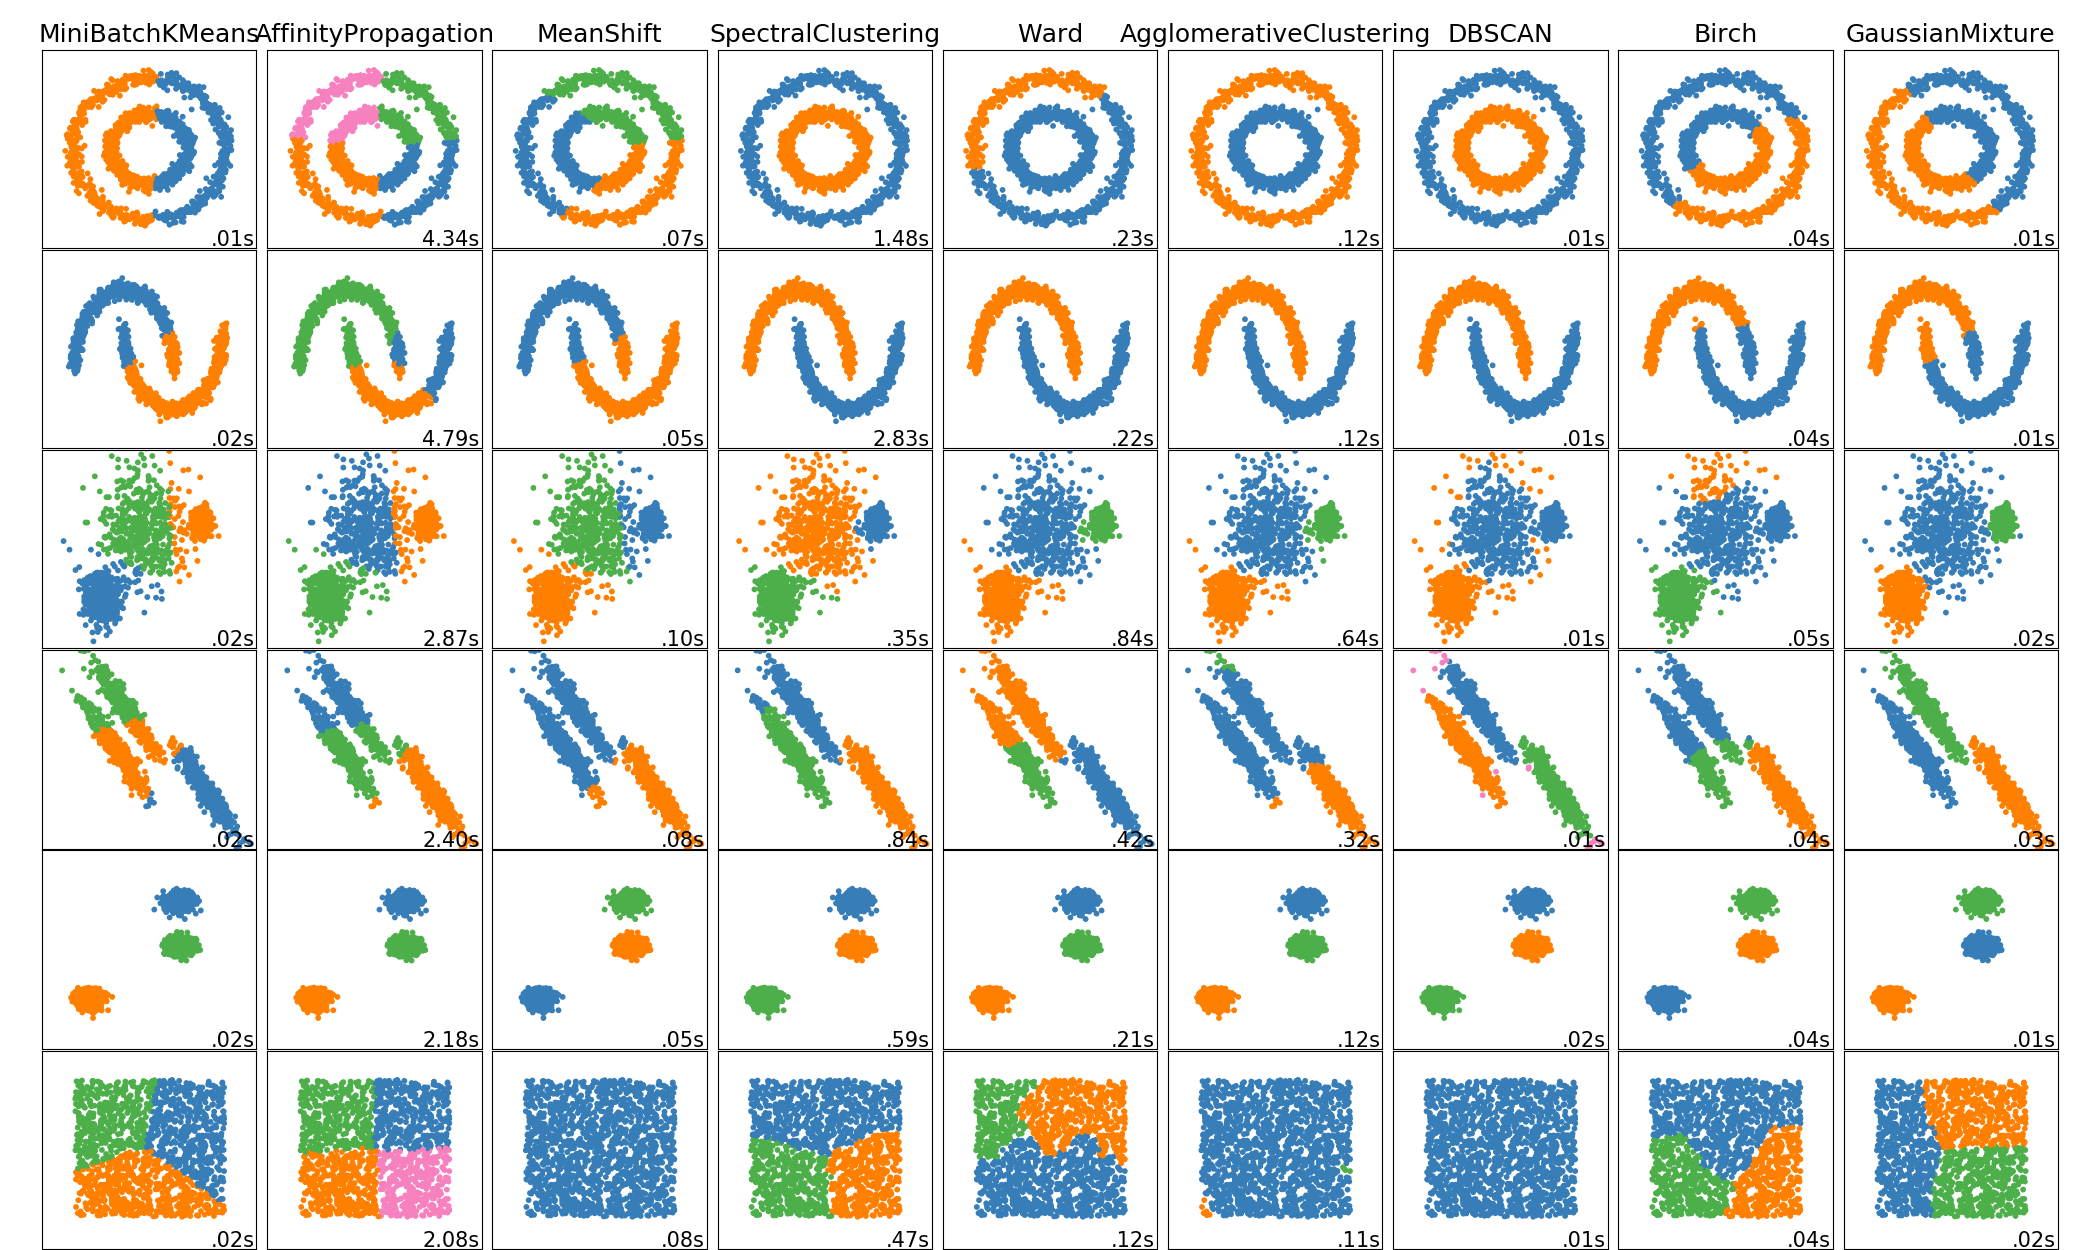
\includegraphics[scale=0.15]{clustering}

\end{frame}




\subsection{Density Models}
\begin{frame}\frametitle{mean-shift clustering}

consider a set of points in two-dimensional space\\
a circular sliding window C centered and radius r as the kernel\\
hill-climbing algorithm that involves shifting this kernel iteratively to a higher density ($\propto$ number of points)  region until convergence\\
At every iteration,\\
- shift the center point to the mean of the points within the window (hence the name)\\
-gradually move towards areas of higher point density\\
- until no longer increase in the density\\
- When multiple sliding windows overlap the window containing the most points is preserved. The data points are then clustered according to the sliding window in which they reside.


\end{frame}


\begin{frame}%\frametitle{meanshift}
\hspace*{-4pt}\makebox[\linewidth][c]{
\begin{tabular}{ccccc}
	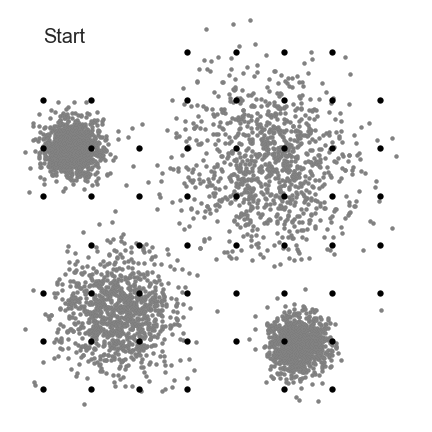
\includegraphics[scale=0.15]{meanshift/meanshift-3}&
	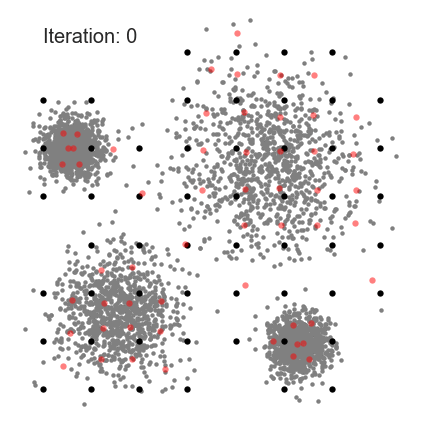
\includegraphics[scale=0.15]{meanshift/meanshift-4}&
	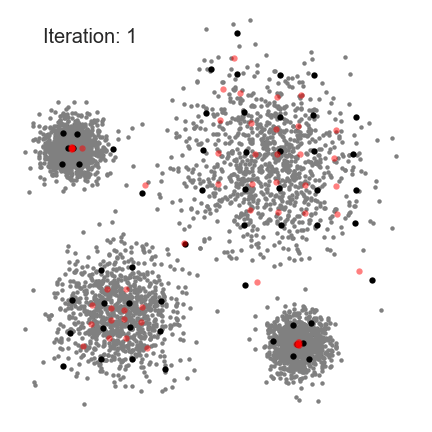
\includegraphics[scale=0.15]{meanshift/meanshift-6}&
	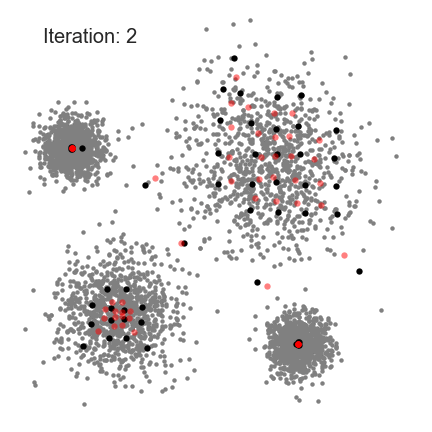
\includegraphics[scale=0.15]{meanshift/meanshift-8}&
	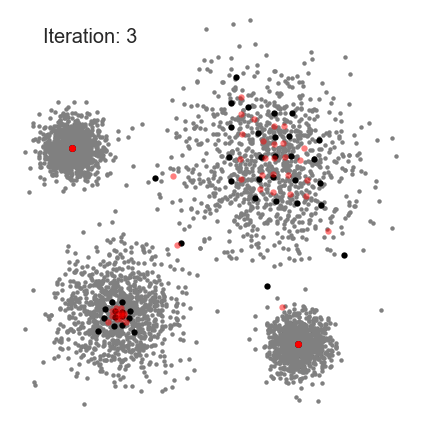
\includegraphics[scale=0.15]{meanshift/meanshift-10}\\
	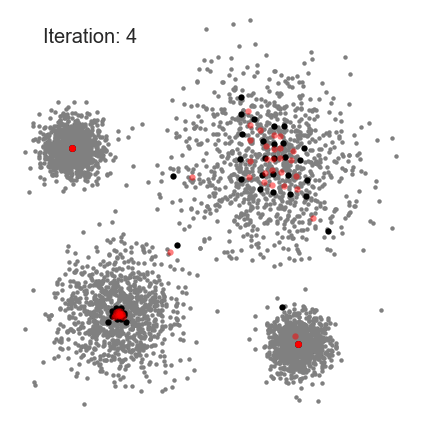
\includegraphics[scale=0.15]{meanshift/meanshift-12}&
	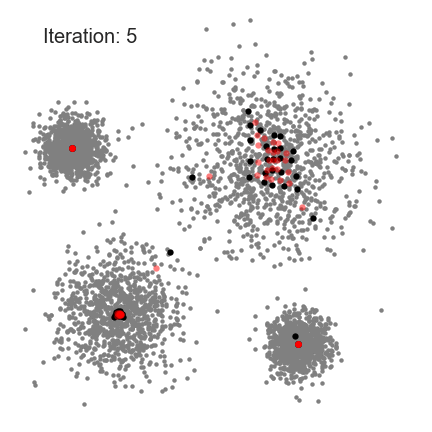
\includegraphics[scale=0.15]{meanshift/meanshift-14}&
	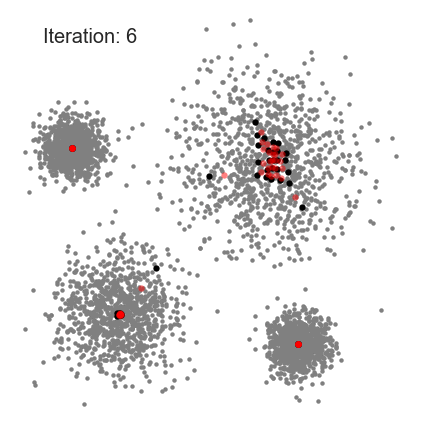
\includegraphics[scale=0.15]{meanshift/meanshift-16}&
	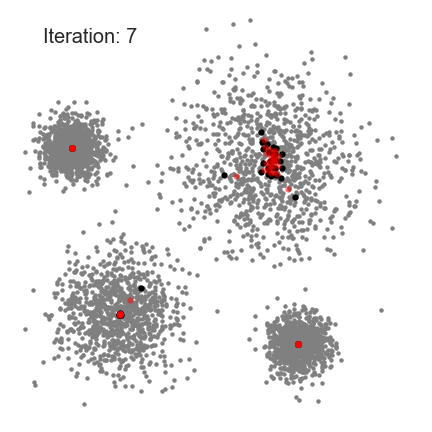
\includegraphics[scale=0.15]{meanshift/meanshift-18}&
	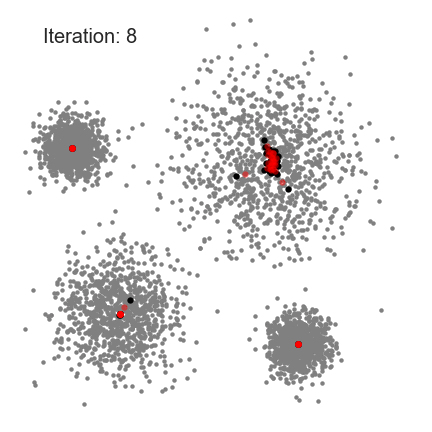
\includegraphics[scale=0.15]{meanshift/meanshift-20}\\
	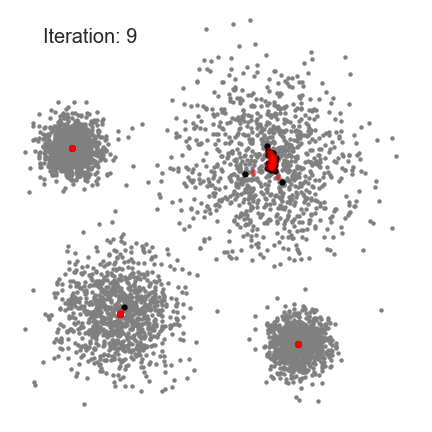
\includegraphics[scale=0.15]{meanshift/meanshift-22}&
	%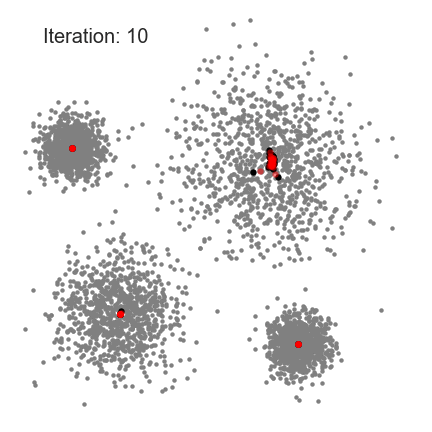
\includegraphics[scale=0.15]{meanshift/meanshift-24}&
	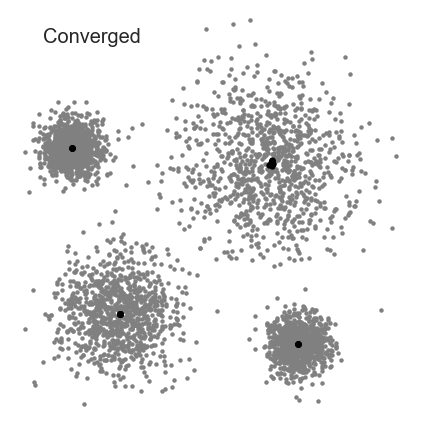
\includegraphics[scale=0.15]{meanshift/meanshift-36}&
	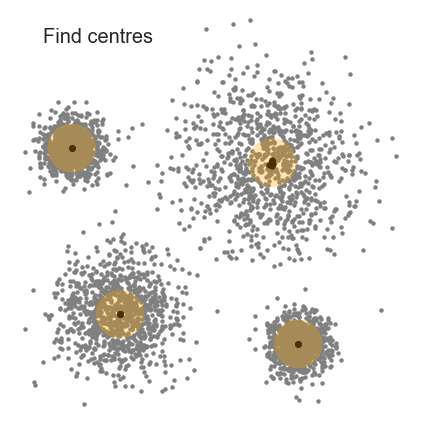
\includegraphics[scale=0.15]{meanshift/meanshift-38}&
	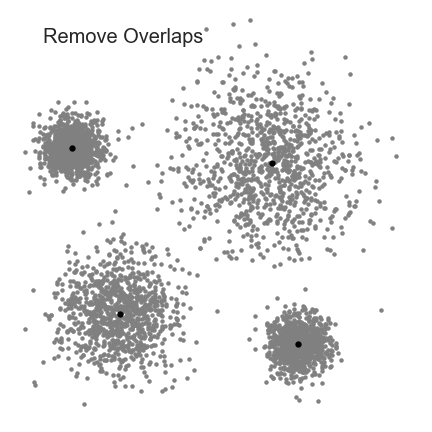
\includegraphics[scale=0.15]{meanshift/meanshift-40}&
	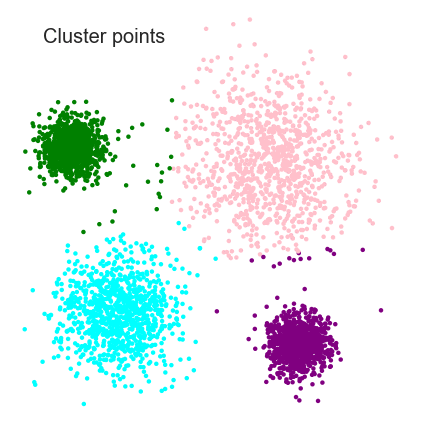
\includegraphics[scale=0.15]{meanshift/meanshift-43}\\
\end{tabular}
}
\end{frame}

\begin{frame}\frametitle{Density-Based Spatial Clustering of Applications with Noise-DBSCAN}
-label all data point to be unvisited. For all unvisited points:
	\begin{enumerate}
		\item All points which are within the $\epsilon$ distance are neighborhood points (part of the same cluster)
		\item If neighborhood points >= minPoints, then the clustering process starts and the current data point becomes the first point in the new cluster
		- Otherwise, mark the point as noise
		- In both cases that point is marked as “visited”
		\item repeated for all of the new points in the cluster group
		\item next an new unvisited point is retrieved and processed
	\end{enumerate}
Since at the end of this all points have been visited, each point will have been marked as either belonging to a cluster or being noise.

\end{frame}


\begin{frame}%\frametitle{dbscan}
\hspace*{-4pt}\makebox[\linewidth][c]{
	\begin{tabular}{cccc}
		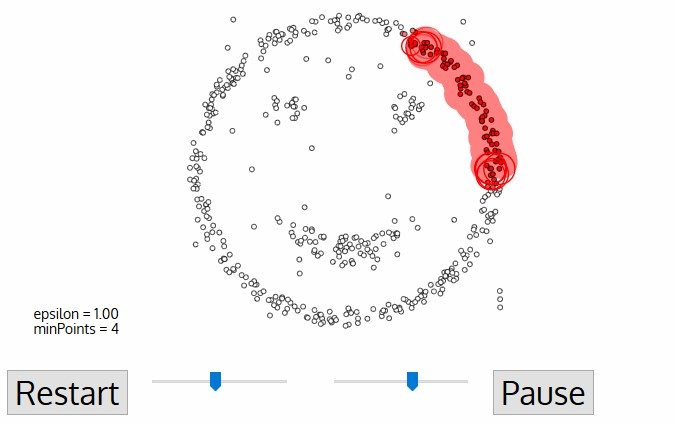
\includegraphics[scale=0.15]{dbscan/1}&
		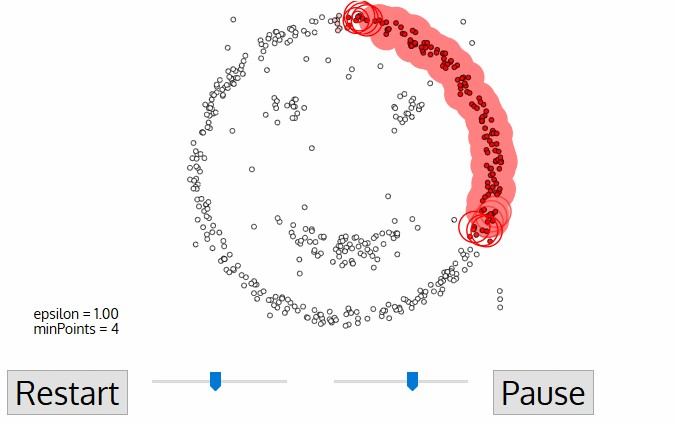
\includegraphics[scale=0.15]{dbscan/11}&
		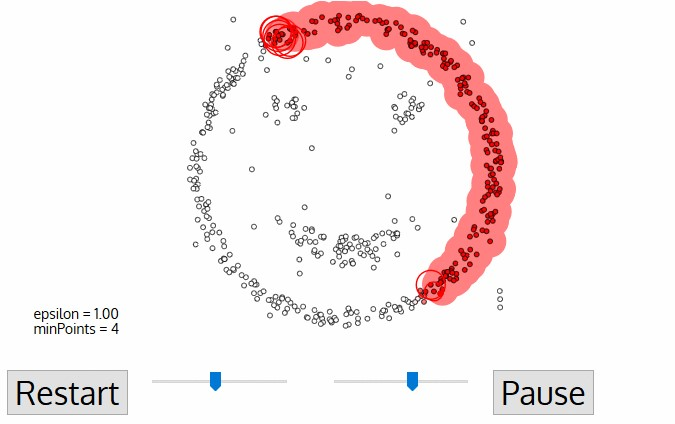
\includegraphics[scale=0.15]{dbscan/2}&
		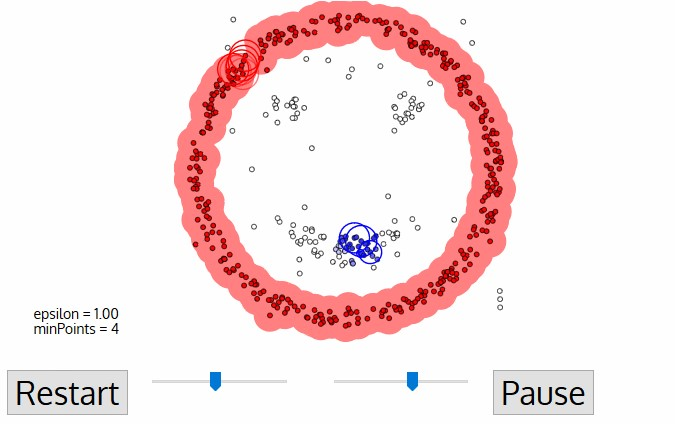
\includegraphics[scale=0.15]{dbscan/3}\\
		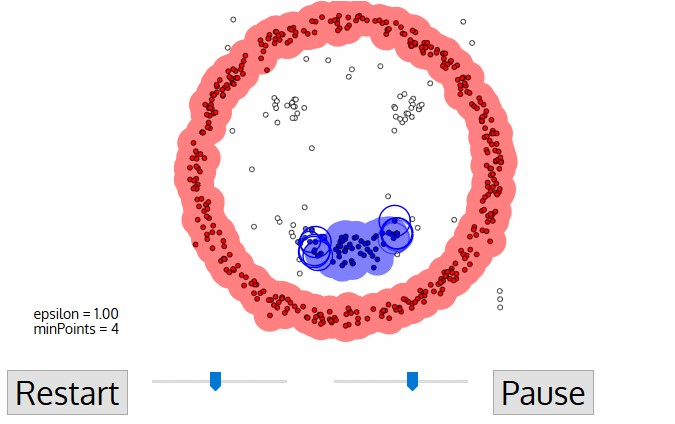
\includegraphics[scale=0.15]{dbscan/31}&
		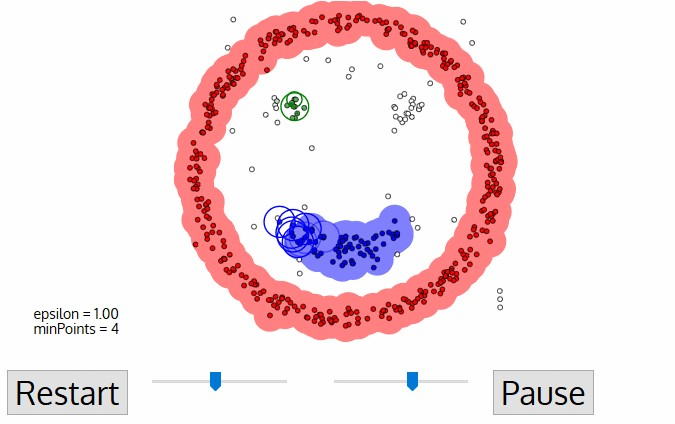
\includegraphics[scale=0.15]{dbscan/4}&
		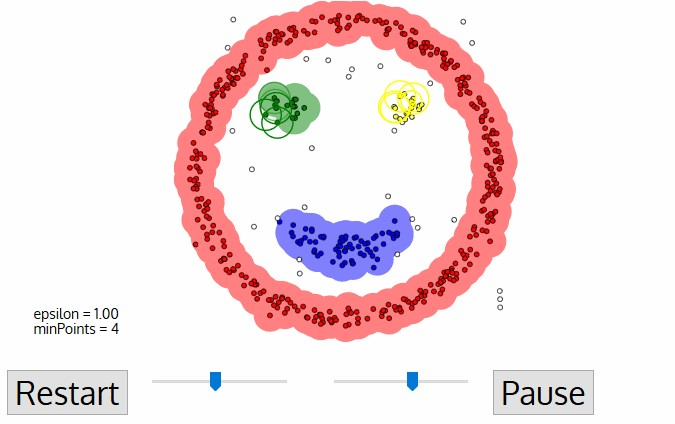
\includegraphics[scale=0.15]{dbscan/5}&
		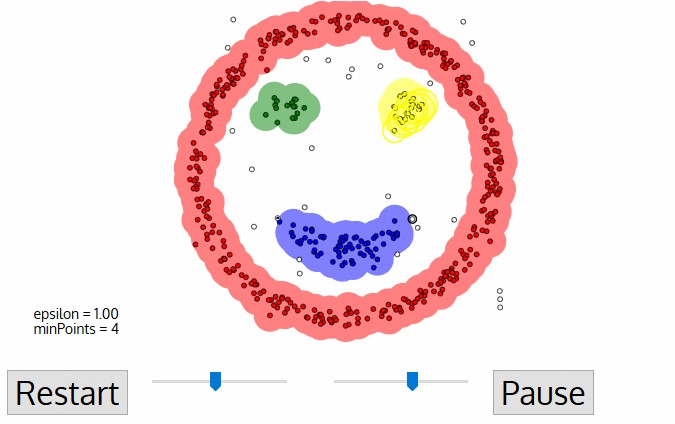
\includegraphics[scale=0.15]{dbscan/6}\\
		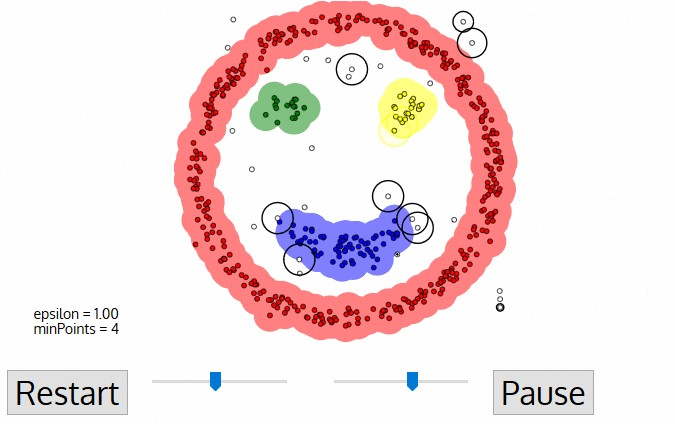
\includegraphics[scale=0.15]{dbscan/7}&
		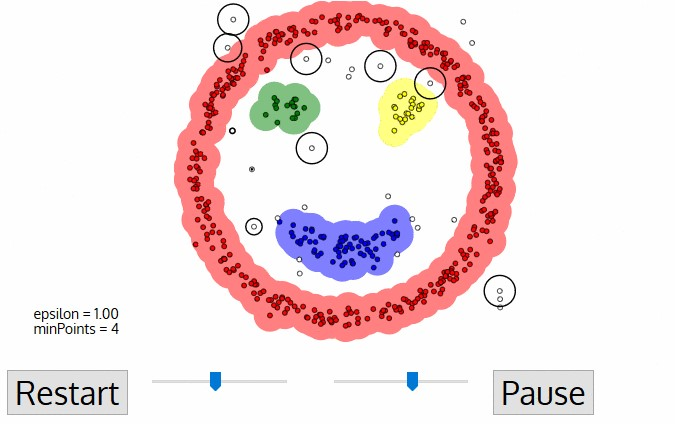
\includegraphics[scale=0.15]{dbscan/8}&
		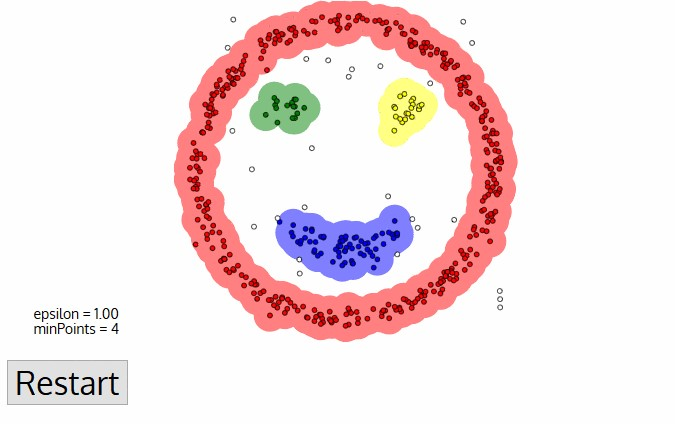
\includegraphics[scale=0.15]{dbscan/9}&
		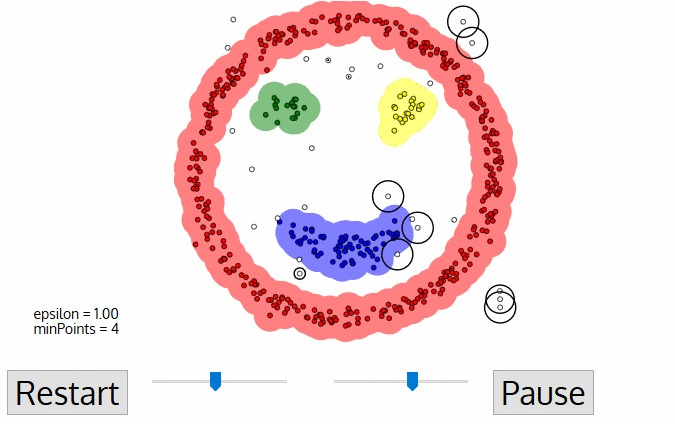
\includegraphics[scale=0.15]{dbscan/10}\\
	\end{tabular}
}
\end{frame}


\begin{frame}\frametitle{Hierarchical DBSCAN - HDBSCAN}
	content...
\end{frame}



\subsection{Distribution Models}
\begin{frame}\frametitle{Gaussian Mixture Models (GMMs)}
Assumption: the data points are Gaussian distributed (parameters: the mean and the standard deviation)! Each Gaussian distribution is assigned to a single cluster.
To find the parameters of the Gaussian for each cluster, use an optimization algorithm called Expectation–Maximization (EM). 

\end{frame}

\begin{frame}\frametitle{Expectation–Maximization (EM) using GMM}
choose num of clusters\\
compute the probability that each data point belongs to a particular cluster. With a Gaussian distribution we are assuming that most of the data lies closer to the center of the cluster.\\
From probabilities $\rightarrow$ recompute set of parameters such that we maximize the probabilities of data points within the clusters\\
We compute these new parameters using a weighted sum of the data point positions, where the weights are the probabilities of the data point belonging in that particular cluster.\\
Repeat till convergence\\

\end{frame}

\begin{frame}%\frametitle{EM}
\hspace*{-4pt}\makebox[\linewidth][c]{
\begin{tabular}{ccccc}
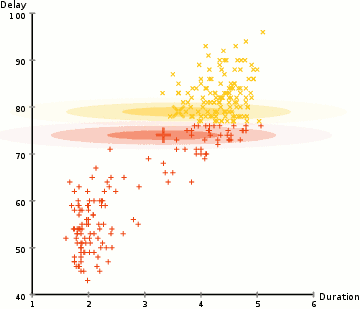
\includegraphics[scale=0.2]{em/frame_00_delay-0}&
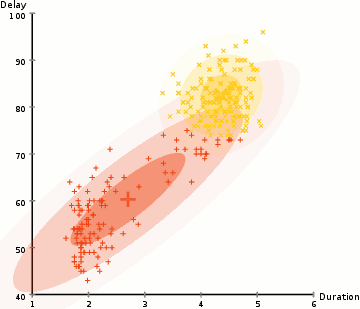
\includegraphics[scale=0.2]{em/frame_01_delay-0}&
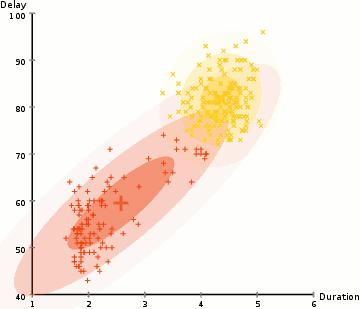
\includegraphics[scale=0.2]{em/frame_02_delay-0}&
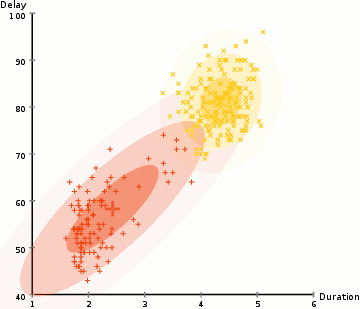
\includegraphics[scale=0.2]{em/frame_03_delay-0}&
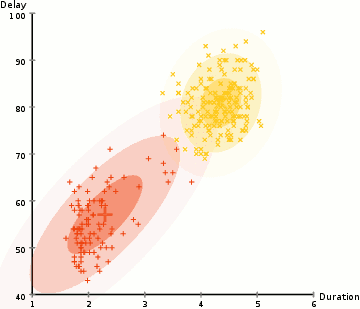
\includegraphics[scale=0.2]{em/frame_04_delay-0}\\
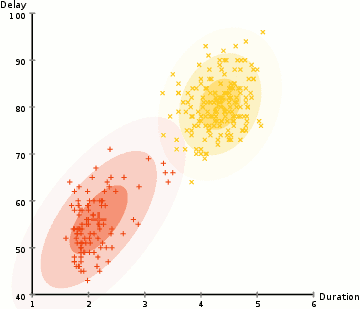
\includegraphics[scale=0.2]{em/frame_05_delay-0}&
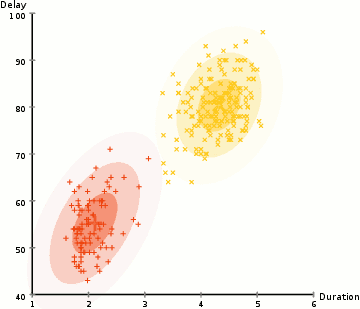
\includegraphics[scale=0.2]{em/frame_06_delay-0}&
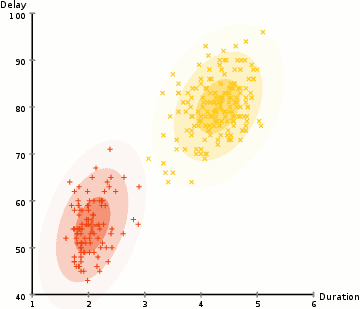
\includegraphics[scale=0.2]{em/frame_07_delay-0}&
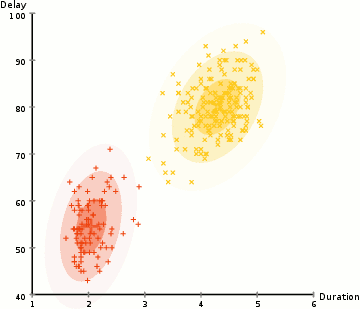
\includegraphics[scale=0.2]{em/frame_08_delay-0}&
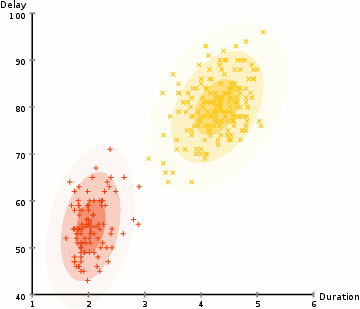
\includegraphics[scale=0.2]{em/frame_09_delay-0}\\
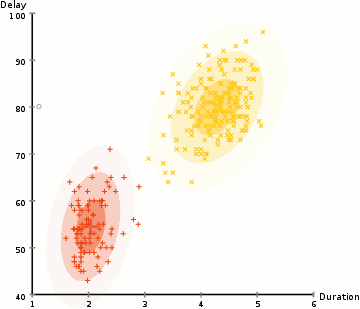
\includegraphics[scale=0.2]{em/frame_10_delay-0}&
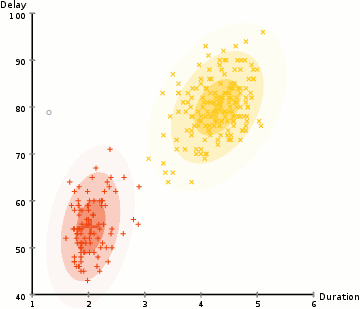
\includegraphics[scale=0.2]{em/frame_11_delay-0}&
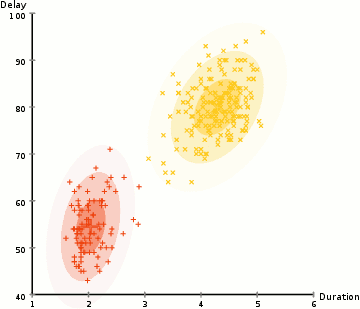
\includegraphics[scale=0.2]{em/frame_12_delay-0}&
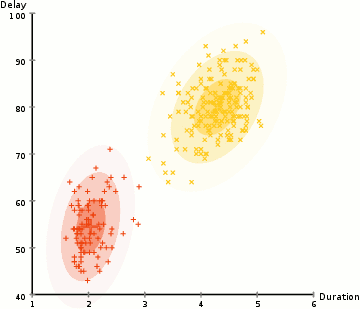
\includegraphics[scale=0.2]{em/frame_13_delay-0}&
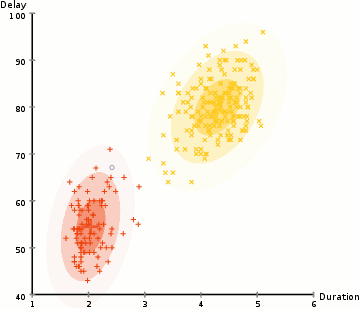
\includegraphics[scale=0.2]{em/frame_14_delay-0}\\
\end{tabular}
}
\end{frame}


\subsection{Centroidal models}
\begin{frame}\frametitle{K means}
iterative clustering algorithm that aims to find local maxima in each iteration\\
take a quick look at the data and choose k (num clusters)\\
assign data points to the cluster $\leftrightarrow$
compute cluster centroid\\
repeat to reduce variation error\\
elbow method
\begin{columns}
	\begin{column}{.5\textwidth}
		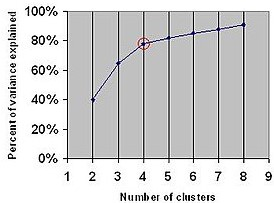
\includegraphics[scale=0.5]{kmeans_1}
	\end{column}
	\begin{column}{.5\textwidth}
		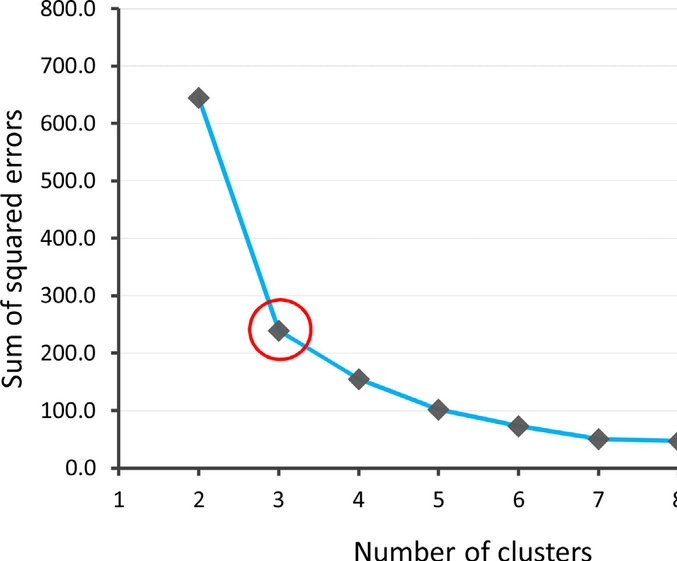
\includegraphics[scale=0.2]{kmeans_2}
	\end{column}
\end{columns}
\end{frame}



\begin{frame}\frametitle{k-median}
\textbf{K median vs kmeans}: instead of recomputing the group center points using the mean (like in K-Means) we use the median vector of the group. This method is \textbf{less sensitive to outliers} (because of using the Median) but is \textbf{much slower for larger datasets as sorting is required} on each iteration when computing the Median vector\\
\textbf{mean-shift vs kmeans}: Instead of selecting the number of clusters as mean-shift automatically discovers this (advantage), the selection of the window size/radius “r” can be non-trivial.

\end{frame}


\begin{frame}\frametitle{kmeans fail}
	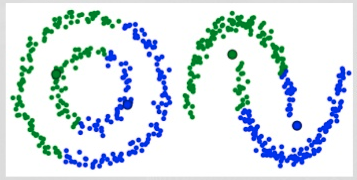
\includegraphics[scale=0.5]{kmeans_fail}\\
	K-Means is actually a special case of GMM in which each cluster’s covariance along all dimensions approaches 0
\end{frame}



\subsection{Connectivity Models}
\begin{frame}\frametitle{Agglomerative Hierarchical Clustering}
The decision of dividing into or merging \textbf{two} clusters is taken on the basis of closeness of these clusters. Metrics for deciding the closeness of two clusters:\\
Euclidean distance: $||a-b||_2=\sqrt{\sum(a_i-b_i)}$\\
Squared Euclidean distance: $||a-b||_2^2=\sum(a_i-b_i)^2$\\
Manhattan distance: $||a-b||_1=\sum|a_i-b_i|$\\
Maximum distance: $||a-b||_{INFINITY} =\max_i|a_i-b_i|$\\
Mahalanobis distance: $\sqrt(a-b)^T S^{-1} (-b)$\\
Maybe, use \textbf{average linkage} which defines the distance between two clusters to be the average distance between data points in the first cluster and data points in the second cluster.

\end{frame}


\begin{frame}\frametitle{hierarchical agglomerative clustering (HAC) or bottom-up}

\begin{enumerate}
	\item Each data point as a single cluster
	\item select a distance metric 
	\item Iterate till convergence\\
	 - combine two clusters with the smallest average linkage
\end{enumerate}



\begin{columns}
	\begin{column}{0.3\textwidth}
		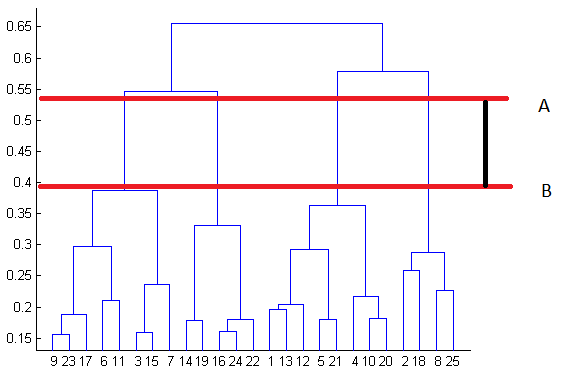
\includegraphics[scale=0.25]{hierarchical}
	\end{column}
	\begin{column}{0.65\textwidth}
		
		The height in the dendrogram at which two clusters are merged represents the distance between two clusters in the data space.\\
		take 4 clusters as the red horizontal line in the dendrogram covers maximum vertical distance AB.\\
		
		
	\end{column}
\end{columns}

\end{frame}













%%%%%%%%%%%%%%%%%%%%%%%%%%%%%%%%%%%%%%%%%%%%%%%%%%%%%%%%%%%%%%%%%%%%%%%%%%%%%%%%%%%%%%%%%%%%%%%%%%%%%%%%%%%%%%%%%%%%%%%%%%%%%%%%%%%%%%%%%%








\section{Analysis}
\subsection{Customer Analysis}

\begin{frame}\frametitle{Churn or Retention Analysis}
Customer Retention Rate: The percentage of customers who repurchase in a given time period compared to an equal and preceding time period\\
Churn Rate: The inverse of Customer Retention Rate, or the percent of users who did not repurchase or whom you lost\\

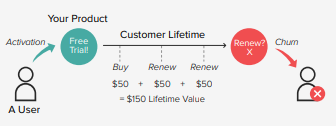
\includegraphics[scale=0.5]{churn}\\
\textbf{proactive churns}: losing customers due to cancellations\\ \textbf{passive churn}: failures to renew\\
\end{frame}


\begin{frame}\frametitle{Cohort Analysis and Life Time Value (LTV)}
	\textbf{LTV}: The expected amount of profit/revenue from a user\\
	CLV = NPV (net present value) of the sum of all future revenues from a customer, minus all costs associated with that customer\\
	\textbf{Why LTV}:
	- Tracking your LTV to Customer Acquisition Cost (CAC) ratio: Companies typically use the 3:1 CAC ratio or Cost Per Acquisition (CPA)\\
	- Evaluating your most valuable marketing channels\\
	- Focus on retaining your most valuable customers\\
	\textbf{Historic CLV}: sum of the gross profit from all historic purchases for an individual customer

	
\end{frame}

\begingroup
\small

\begin{frame}

	\begin{table}
		\begin{tabular}{llll}
			%\hline
			\multicolumn{2}{c}{Avg Order Value, AOV = $\frac{Revenue}{Orders}$};
			& \multicolumn{2}{c}{Avg Purchase Rate = $\frac{Orders}{NumCustomers}$} 
			\\ \hline
			\multicolumn{3}{c}{Avg Customer Value = $\frac{Avg Purchase Val}{Avg Purchase Rate}$}
			& \multirow{2}{*}{gives LTV}
			\\ %\hline
			\multicolumn{3}{c}{Avg Customer Lifespan = $\frac{Sum Customer Lifespans}{Num Customers}$}
			& \\ \hline
			\multirow{5}{*}{LTV = }
			& \multicolumn{3}{l}{Avg Customer Value X Avg Customer Lifespan}
			\\ 
			& \multicolumn{3}{l}{ARPU X $\sum_{n=0}^{N}(1-CR)^t$ .... [N=num months to examine]}
			\\
			& \multicolumn{3}{l}{ARPU/$CR_n$ ...[ARPU=Avg rev per User, for n months]}
			\\
			& \multicolumn{3}{l}{ARPU/$CR_n$ x DR ......... [for variable churn \& n months]}
			\\
			& \multicolumn{3}{l}{ASP/CR + m(1-CR)/$CR^2$ ... [for account expansion]}
			\\ \hline
			\multirow{3}{*}{CLV = }
			& \multicolumn{3}{l}{AGM x $\sum_{0}^{numTransactions} Transaction$ [AGM=Avg Gross Margin]}
			\\
			& \multicolumn{3}{l}{(($T_{avg}xAOV$)AGM)ALT =GML(gross margin per user lifespan)}
			\\
			& \multicolumn{3}{l}{GML(R/(1+D-R)); [account expansion]}
			\\
			\hline
		\end{tabular}
	\end{table}


CR=Churn rate; ASP=Avg Selling Price; m=$\uparrow$ARPU/user/month;\\
T\_avg = avg monthly transactions; ALT=avg User Lifespan (in months)\\
D=monthly discount rate; R=monthly retention rate; 
DR=Discount Rate to adjusts for mix churn (Annual Renewals, Constant, Declining and Cliff patterns)

\end{frame}

\endgroup

\begin{frame}
	Steps to LTV:
	\begin{itemize}
		\item Normalizing to Acquisition Date: Bin users into buckets like Day 0, Day 1, Day 2 or Week 0, Week 1, Week 2, and so on.
		\item Normalized to a Closed Time Limit: Broader questions  “What is my total CLTV,” should be replaced with “What is our 3-year or 5-year LTV?” \& should be based on:
		\begin{enumerate}
			\item Average Customer Lifespan
			\item Customer Retention Rate
			\item Churn Rate: The inverse of Customer Retention Rate.
			\item Time to General Profitability Against Acquisition Costs: If your business is a “Loss Leader” Model this time may be a longer length than businesses with lower acquisition costs and lower profitability.
			\item Rate of Discount		
		\end{enumerate}

	\end{itemize}
\end{frame}

\begin{frame}\frametitle{Types of churn and LTV}
	\begin{itemize}
		\item Annual Renewals: larger churn at each contract renewal.
		\item Cliff churn: majority of the churn within the first month, and then a small constant churn thereafter.
		\item Constant: steady, constant churn rate (shown as 3.5\%).
		\item Declining: churn rate starts at zero, increases each month.
	\end{itemize}
	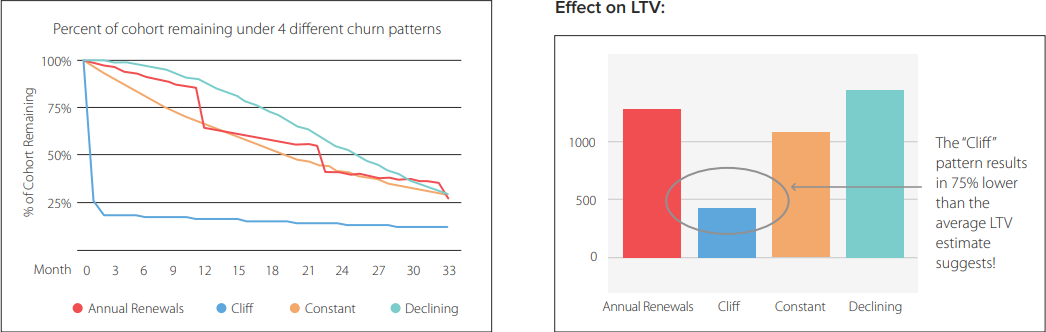
\includegraphics[scale=0.4]{churnltv}
\end{frame}

\begin{frame}\frametitle{Survival Analysis}
content...
\end{frame}

\begin{frame}\frametitle{Sentiment Analysis}
content...
\end{frame}

\begin{frame}\frametitle{Propensity of Cross-sell}
content...
\end{frame}


\subsection{Trend Analysis}


\subsection{Other Analysis}
\begin{frame}\frametitle{Whale Curve Analysis}
	\textbf{Pareto Principle}: for many events, roughly 80\% of the effects come from 20\% of the causes\\
	
\end{frame}

\begin{frame}\frametitle{"Loss Leader” Model}

"Loss Leader” Model, where you introduce new customers at a high cost in the hope of building a customer base or securing future revenue? 

\end{frame}

\begin{frame}
	Thank You!
\end{frame}

\end{document}